\section{提案システム}
%第\ref{sec:related-works}で述べたように,これまでに提案されてきた検知に基づくDNS Tunneling対策には,Low Throughput手法および転送頻度を下げる手法に対して,検知が困難であるという課題がある.
%他方,新しいアーキテクチャに基づく名前解決システムには,マイグレーションの課題が残留している.
本章では,提案システムについて説明する.
はじめにシステムの概要と目的を示す.
次に,システムの詳細に関して,アーキテクチャ・動作メカニズム・プロトコル・スケーラビリティを順に説明する.

\subsection{フラットな名前空間に基づく名前解決システム : REFRES}
本節では,システムの概要について説明する.

REFRES(REcorded inFormation REsolution System)は,フラットな名前空間においてハッシュ値の範囲に基づきゾーンを分割し,そのゾーンを管理する主体として既存システムのTLDを割り当てることで,名前解決の手続きにおけるノードをクライアントとゾーン管理ノードのみに限定させた名前解決システムである.
REFRESでは,ドメイン名``www.example.com"のAレコードやドメイン名``www.example.com"のTXTレコードなど全てのレコード情報をフラットな名前空間上で管理する.
また,ドメイン名とリソースレコードタイプもしくはIPアドレスとリソースレコードタイプから算出されるハッシュ値を識別子とすることでレコード情報へのアクセスを実現する.
このようにして,REFRESにおけるクライアントは,レコード情報を保持するノードを一意に特定することができる.
具体的なレコード情報は,ゾーンを管理するサーバノードに階層的に連結したノードのよって作成・更新・破棄される.
レコード情報を操作する際には,事前に認証局との認証手続きをすることで,レコード情報の信頼を保証する.
最終的にREFRESでは,クライアントからの名前解決リクエストと偽装して送信される特定の権威サーバ指向の悪性クエリが発生する仕組みを抑止する.
REFRESの特徴を以下に示す.
\begin{itemize}
 \item フラットな名前空間
 \vspace{-3mm}
 \item ハッシュ値の範囲に基づくゾーニング
 \vspace{-3mm}
 \item レコード情報の操作と提供・管理の機能分離
 \vspace{-3mm}
 \item レコード情報に対する識別子の導入
 \vspace{-3mm}
 \item 全てのレコード情報が認証済み
\end{itemize}

\begin{figure}[t]
 \centering
 \label{fig:abstruct-REFRES-architecture}
 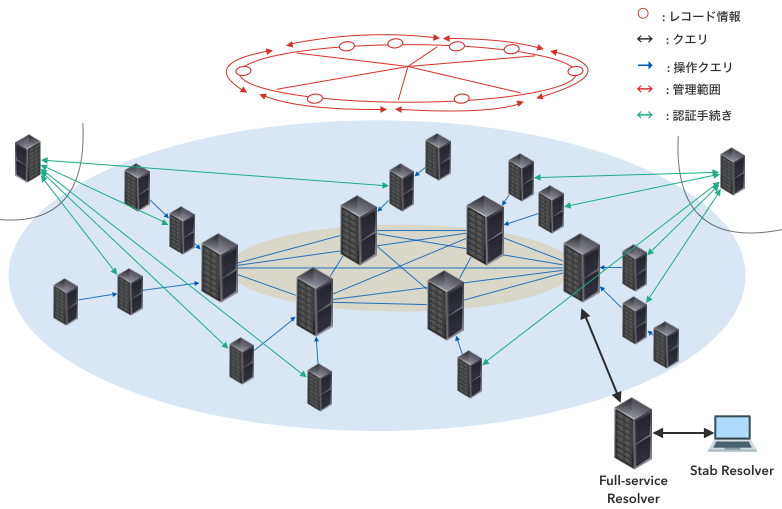
\includegraphics[scale=0.5]{figure/abstruct-architecture.png}
 \caption{REFRESの全体図}
\end{figure}


\subsection{システムデザイン}
REFRESのアーキテクチャは,全体として既存のDNS同様のクライアントサーバアーキテクチャを継承する.
サーバは,従来のような階層構造ではなく,256bitの名前空間にフラット
のハッシュテーブルの特定範囲をゾーンとするサーバ同士が連携する
フルメッシュネットワークのP2Pアーキテクチャによるハイブリッドに構成される.
は,サーバ同士が相互連携するサーバ群とクライアントで構成されるクライアントサーバアーキテクチャで動作する.
REFRESにおいて,スタブリゾルバとフルサービスリゾルバとの間の手続きは,既存のDNSと変わらない.
しかし,REFRESのサーバは,フルメッシュのネットワーク基盤のもとで各サーバが相互に連携することで,リソース情報を分散して管理する.
%既存のDNSにおける名前解決の仕組みでは,階層的なドメイン構造に基づきルートから順に権威サーバに対し再帰的に問い合わせていくことで,スタブリゾルバからの問い合わせレコード情報を保持するサーバのアドレスを特定する.
REFRESにおけるレコード情報は,QNAMEとレコードタイプを引数として,ハッシュ関数によって算出されるコンテンツIDがシンボルとして紐づけられる.

全てのフルサービスリゾルバは,シンボルとそのシンボルに紐づいたレコード情報を管理するサーバを対応づけた表を保持し,この対応表に基づきコンテンツIDからサーバを一意に特定する.
複数のサーバが,アルファベットおよび数字の順序(a $\rightarrow$ z, 0 $\rightarrow$ 9)で並んだハッシュテーブルの連続した範囲を管理し合い,担当の範囲下にあるコンテンツIDに紐づいたレコード情報を担当サーバが管理する.
対応表~\ref{tab:hash-management}には,どこからのどこまでのハッシュテーブルの範囲をどのサーバが管理するのかについて記述されている.
\begin{table}[htb]
 \caption[マネージャとゾーンの対応表]{マネージャの情報とそのマネージャが管理するゾーンが記載された対応表の例}
 \centering
  \begin{tabular}{lrl}
    \toprule
		\multicolumn{1}{c}{\textbf{ゾーン}} & \begin{tabular}{c}\textbf{マネージャ}\\\textbf{アドレス}\end{tabular} & \multicolumn{1}{c}{\textbf{ドメイン}} \\
    \midrule
    (000…00, 2zz…zz) & 192.35.51.30 & com.  \\
		\multicolumn{1}{c}{...} & \multicolumn{1}{c}{...} & ... \\
    (500…00, 6zz…zz) & 192.5.6.30 & net. \\
		\multicolumn{1}{c}{...} & \multicolumn{1}{c}{...} & ... \\
    (b00…00, czz…zz) & 199.249.112.1 & org. \\
		\multicolumn{1}{c}{...} & \multicolumn{1}{c}{...} & ... \\
    (n00…00, mzz…zz) & 199.254.31.1 & info. \\
		\multicolumn{1}{c}{...} & \multicolumn{1}{c}{...} & ... \\
    (y00…00, zzz…zz) & 194.0.0.53 & arpa. \\
    \bottomrule
  \end{tabular}
 \label{tab:hash-management}
\end{table}

フルサービスリゾルバはQNAMEとリソースレコードタイプをキーとしてサーバに問い合わせるバリューが応答されるKVSモデルに基づく名前解決システムである.
QNAMEとリソースレコードタイプに基づき生成されるハッシュ値をキー,分散ハッシュテーブル上で保存されているレコード情報をバリューとするKVSモデルに基づく名前解決システムである.
REFRESでは,従来のDNSのエコシステムの内,スタブリゾルバからリカーシブサーバまでの手続きを継承することで,エッジノードにおけるシステムのマイグレーションに伴う課題を軽減する.
全てのレコード情報は,レコードタイプとドメイン名もしくはIPアドレスの文字列和(rtype+domain, rtype+ipaddress)をハッシュ関数に適用して算出されるハッシュ値をコンテンツIDとして,レコード情報に紐づけられる.
スタブリゾルバは既存のDNSと変更はなく,DNSクライアントとして,名前解決を依頼する主体として位置づくノードである.
リカーシブサーバは,スタブリゾルバからの問い合わせに対してリソース情報を保持する主体に代理的に問い合わせ機能と,問い合わせた情報を一定期間キャッシュするキャッシュサーバとして機能するノードである.
既存のDNSにおける権威サーバは,リカーシブサーバからの問い合わせに応答するマネージャと,リソース情報について作成・消去および更新などの操作をするプロバイダの二つに分けられる.
REFRESにおいて,リソース情報は,オブジェクト(object)とリソースレコードタイプ(rtype)を引数とするハッシュ関数から算出されるコンテンツIDが紐づけられ,そのコンテンツIDに基づきハッシュ空間上に対応づけられる.
各マネージャは,ハッシュテーブル全体のうち連続した幾らかの管理範囲が割り当てられ,範囲下にあるコンテンツIDに基づいたリソース情報を保存・管理する.
このようにして,リソース情報は,特定の範囲ごとに分割されたハッシュテーブルにて分散的に管理される.
マネージャ同士は,フルメッシュなネットワーク構造で接続し合い,各マネージャには地理的・意味的に類似なプロバイダが階層的な序列に基づき接続される.
プロバイダからリソース情報への操作リクエストがあった際には,リソース情報のコンテンツIDを算出し,そのIDが含まれるハッシュ空間を管理する担当マネージャに操作依頼を転送し,受け取った担当マネージャは直ちに,リソース情報への操作を実行する.



\subsection{レコード情報に対する操作メカニズム}
\subsection{ハッシュ範囲に対する管理ノードの対応表}
\subsection{認証に基づくレコード情報のストア}
\subsection{リソースレコード}
本節では,DNS Infiltrationに対応するため,リソースレコードを再定義する.
\subsection{スケーラビリティ}
%ハッシュテーブルのレプリケーション手法
%特定のハッシュ範囲を管理するノードは,複数用意させ,そのアドレスを対応表に明記し,ストアする際にその全てのレプリケーションサーバにストアリクエストする
